\documentclass[11pt, a4paper]{article}

% --- ATS & Encoding Safety (CRITICAL) ---
\input{glyphtounicode}
\pdfgentounicode=1
\usepackage[T1]{fontenc}
\usepackage[utf8]{inputenc}
\usepackage[scaled]{helvet}
\renewcommand{\familydefault}{\sfdefault}

% --- Packages ---
\usepackage[
    ignoreheadfoot,
    top=1.27cm,
    bottom=1.27cm,
    left=1.27cm,
    right=1.27cm,
    footskip=0.8cm,
]{geometry}
\usepackage{titlesec}
\usepackage{enumitem}
\usepackage{fontawesome5}
\usepackage{xcolor}
\usepackage{graphicx}
\usepackage{hyperref}
\usepackage{needspace}
\usepackage{accsupp}

% --- Color Definitions ---
\definecolor{primaryColor}{RGB}{0,79,144}
\definecolor{darkGray}{RGB}{60,60,60}

% --- Hyperlinks ---
\hypersetup{
    colorlinks=true,
    urlcolor=primaryColor,
    linkcolor=primaryColor,
    pdfborder={0 0 0}
}

% --- Section Formatting ---
\titleformat{\section}
    {\large\bfseries\color{primaryColor}\uppercase}
    {}{0em}
    {}[\titlerule]
\titlespacing{\section}{0pt}{12pt}{8pt}

% --- List Formatting ---
\setlist[itemize]{
    leftmargin=*,
    label={\small\textbullet},
    nosep,
    topsep=4pt,
    itemsep=3pt
}

% --- Custom Commands ---
\newcommand{\entry}[4]{
    \textbf{#1} \hfill \textbf{#2} \\
    \textit{#3} \hfill \textit{#4}
}

% --- ATS-Safe Icon Command ---
\newcommand{\safeicon}[2]{%
    \BeginAccSupp{method=pdfstringdef,ActualText={#1: }}%
    #2%
    \EndAccSupp{}%
}

\begin{document}

% --- HEADER (Dubai Standard) ---
\begin{center}
    \begin{minipage}[c]{0.72\textwidth}
        \raggedright
        {\Huge\textbf{\color{primaryColor}Razim Manzoor}} \\[6pt]
        \textbf{Business Analyst | Data \& AI Analytics | Automation} \\[4pt]
        
        \safeicon{Location}{\faMapMarker*} Dubai, UAE \quad
        \safeicon{Phone}{\faPhone} +971 50 300 1697 \quad
        \safeicon{Email}{\faEnvelope} \href{mailto:manzoorrazim@gmail.com}{manzoorrazim@gmail.com} \\
        \safeicon{LinkedIn}{\faLinkedin} \href{https://www.linkedin.com/in/razim-manzoor}{linkedin.com/in/razim-manzoor} \\[8pt]
        
        \small
        \textbf{Nationality:} Indian \quad | \quad \textbf{Visa Status:} Visit Visa (Available Immediately) \\
        \textbf{Date of Birth:} 25 May 2000 \quad | \quad \textbf{Marital Status:} Single
    \end{minipage}%
    \hfill
    \begin{minipage}[c]{0.25\textwidth}
        \raggedleft
        \IfFileExists{profpic.jpeg}{
            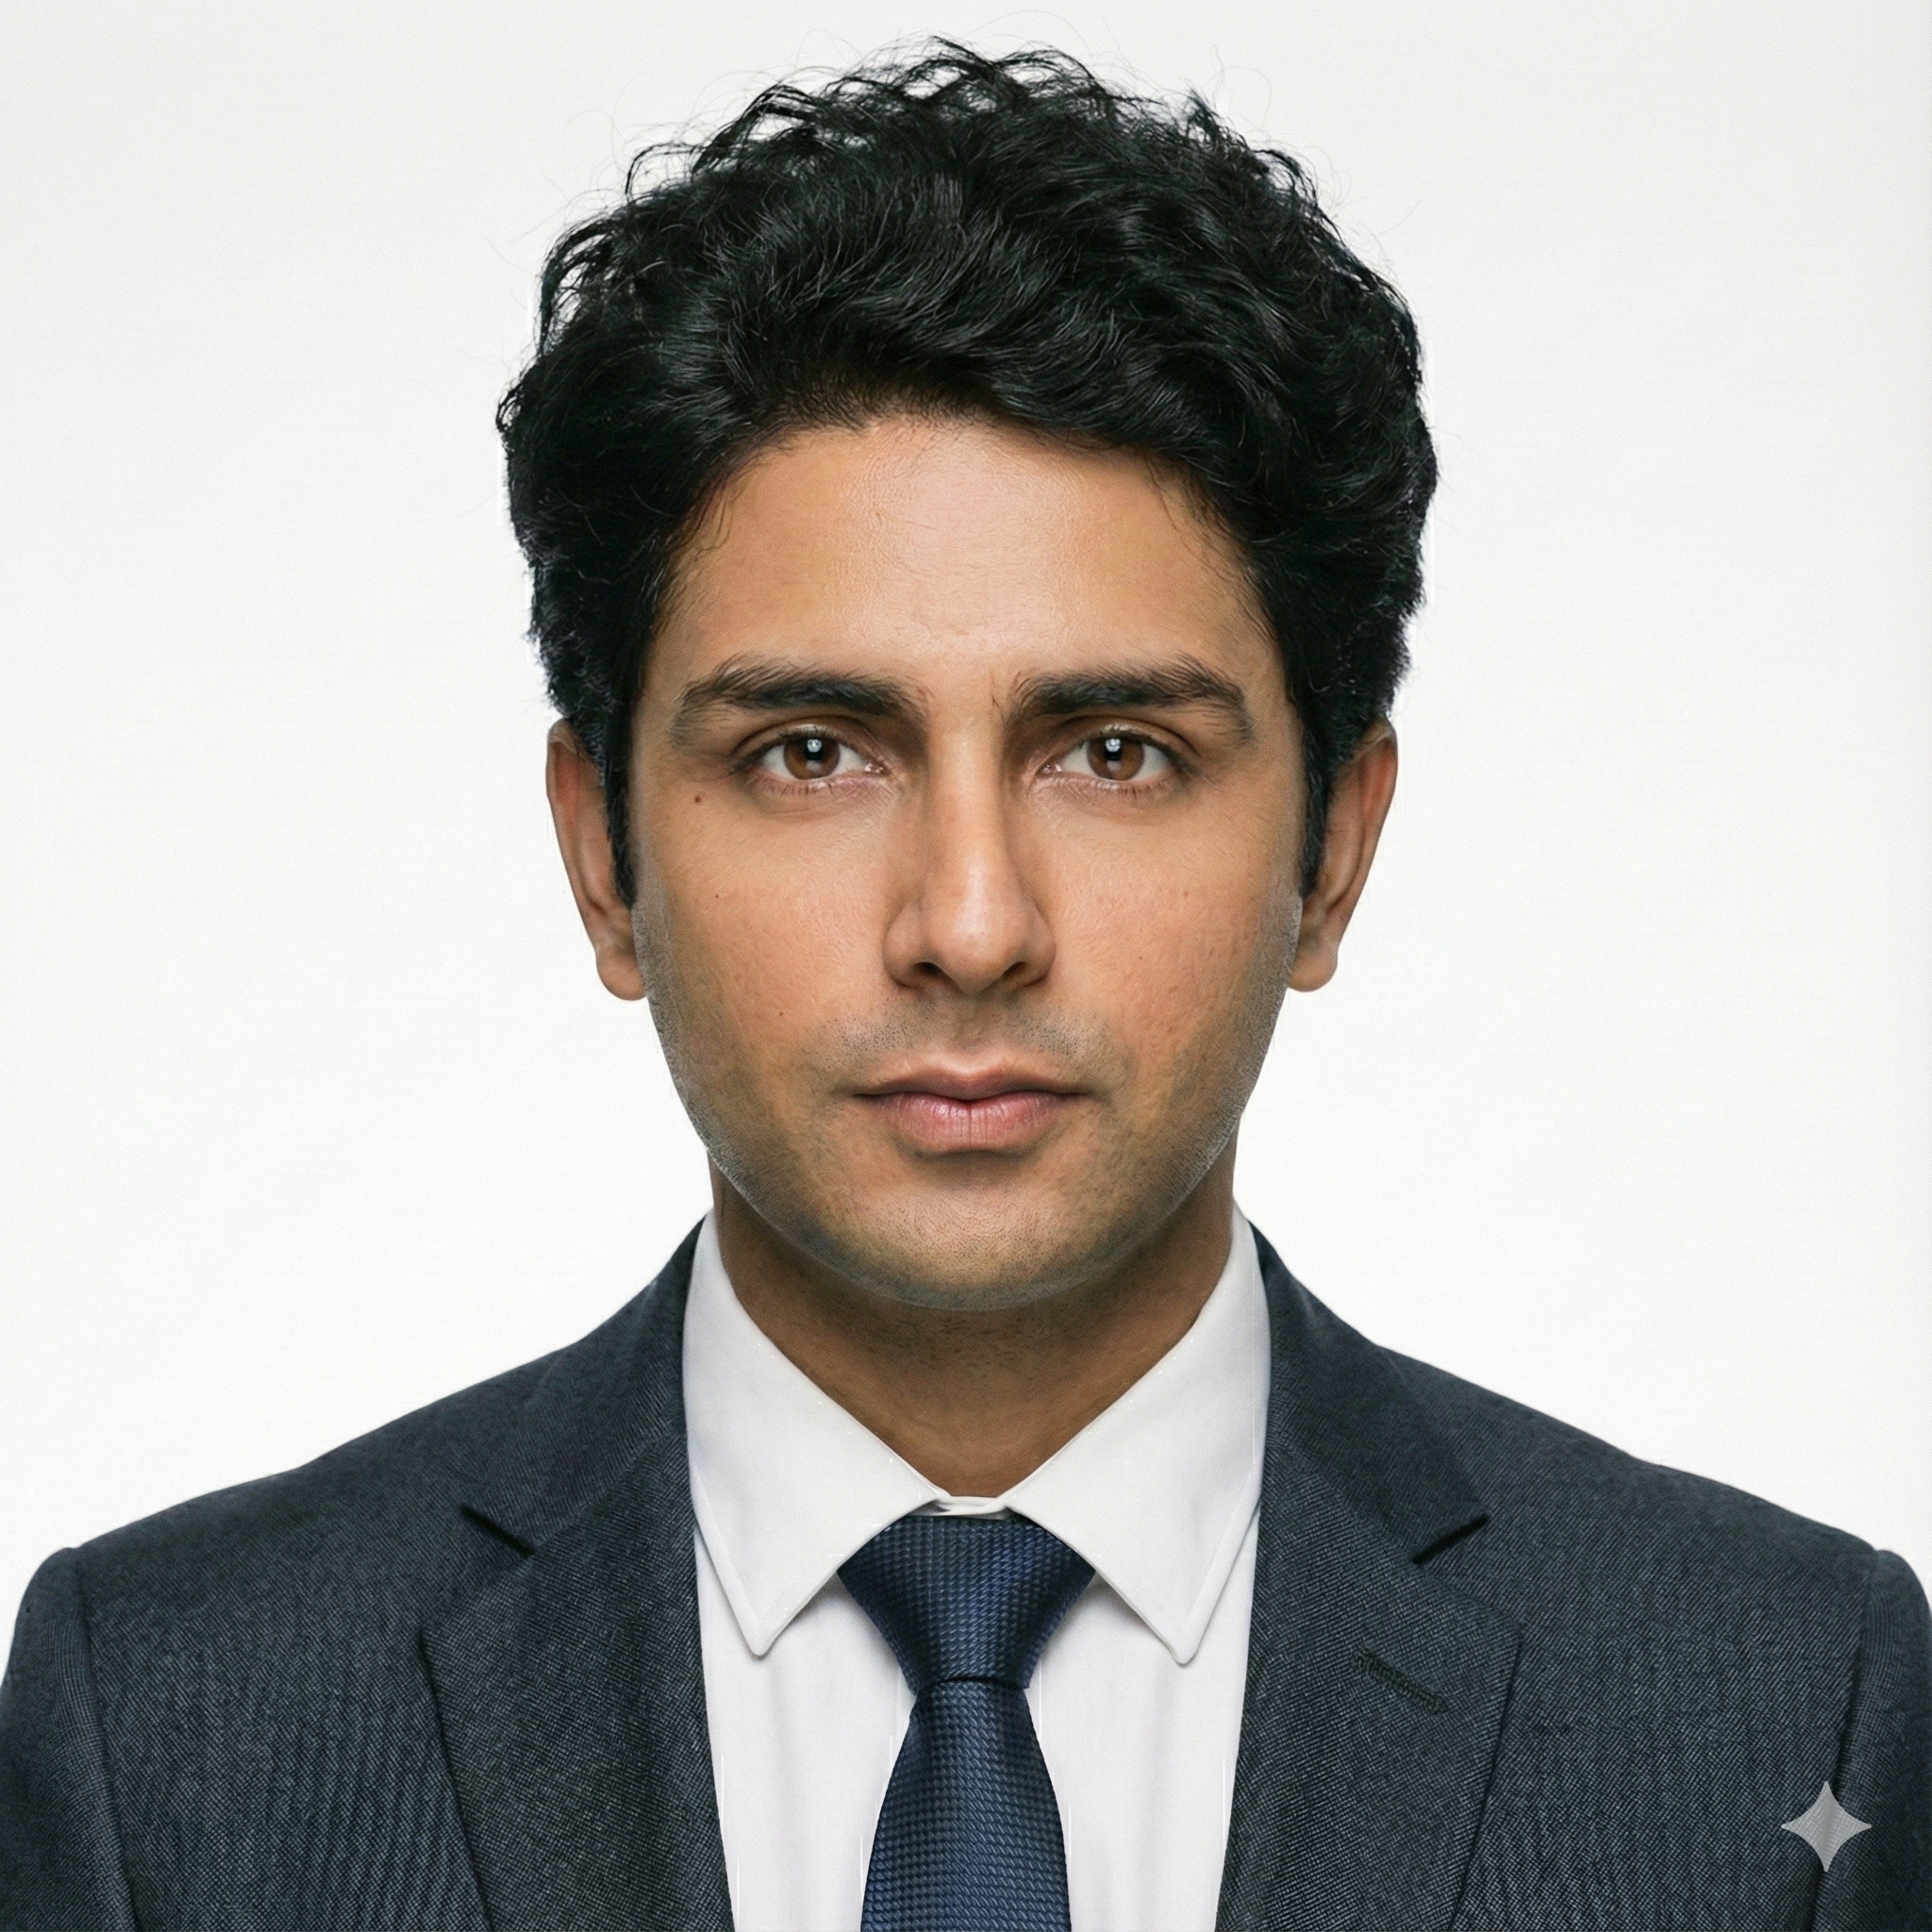
\includegraphics[width=3cm, keepaspectratio]{profpic.jpeg}
        }{
            \fcolorbox{gray}{white}{\parbox[c][3.5cm][c]{3cm}{\centering\tiny Photo Not Found}}
        }
    \end{minipage}
\end{center}

\vspace{0.2cm}

% --- PROFESSIONAL SUMMARY ---
\section{Professional Summary}
MBA-qualified Business and Data Analyst with experience across \textbf{digital transformation},
\textbf{data analytics}, and \textbf{AI-enabled solutions}. Strong ability to translate business
requirements into analytical and automated solutions using Power BI, Python, SQL, and workflow
automation tools. Hands-on exposure to \textbf{Generative AI} (RAG, LLMs) and business intelligence
dashboards to improve operational efficiency, reporting accuracy, and decision-making.

% --- CORE COMPETENCIES ---
\section{Core Competencies \& AI Fluency}
\begin{itemize}[leftmargin=0pt, label={}]
    \item \textbf{Business Strategy:} Strategic Planning, KPI Analysis, Process Mining, ROI Assessment, Market Segmentation, Requirement Gathering, Stakeholder Management.
    \item \textbf{Data Ecosystem:} Power BI (Advanced DAX), Python (Pandas, Scikit-learn), SQL, Azure, Tableau, Advanced Excel.
    \item \textbf{AI \& Automation:} Generative AI (LLMs), Retrieval-Augmented Generation (RAG), Prompt Engineering, AI Agents, Workflow Automation (Power Automate, UiPath).
\end{itemize}

% --- PROFESSIONAL EXPERIENCE ---
\section{Professional Experience}

\entry{Data Strategy Associate (Industrial Trainee)}{Jun 2024 -- Mar 2025}{Luminar Technolab}{Kochi, India}
\begin{itemize}
    \item \textbf{End-to-End Development:} Spearheaded the development of a portfolio of
    \textbf{scalable data and analytics solutions}, utilizing Python, SQL, and Deep Learning
    to address complex business logic challenges.
    
    \item \textbf{Revenue Strategy:} Engineered a predictive customer segmentation model
    using Machine Learning that identified a \textbf{projected 15\% revenue uplift opportunity},
    delivering actionable insights to sales teams.
    
    \item \textbf{Business Intelligence:} Managed the migration of legacy reporting into
    real-time \textbf{Power BI dashboards}, reducing executive reporting latency by 95\%
    (from 3 days to 2 hours).
    
    \item \textbf{Capability Validation:} Achieved an A+ grade in Data Science \& Python
    implementation, demonstrating proficiency in deploying analytical and AI models for
    enterprise use cases.
\end{itemize}

\vspace{8pt}

\entry{Associate AI and Data Analytics Engineer}{Nov 2023 -- May 2024}{Resemble Systems}{Kochi, India}
\begin{itemize}
    \item \textbf{Digital Transformation:} Led a finance automation initiative using
    \textbf{Power Automate}, streamlining invoice processing workflows and reducing manual
    data entry effort by \textbf{45\%}.
    
    \item \textbf{Process Optimization:} Conducted \textbf{process mining} to map operational
    workflows, identify bottlenecks, and support RPA-driven cycle time improvements of
    \textbf{20\%}.
    
    \item \textbf{Workforce Analytics:} Designed HR analytics dashboards to visualize
    attrition and engagement KPIs, enabling data-driven workforce planning.
    
    \item \textbf{Cloud Integration:} Collaborated on Azure-based deployments to ensure
    scalable and secure automation solutions.
\end{itemize}

% --- EDUCATION ---
\section{Education}

\entry{Master of Business Administration (MBA)}{2021 -- 2023}{JAIN University}{India}
\begin{itemize}
    \item \textit{Specialization:} Data Science \& Analytics
    \item \textit{Relevant Coursework:} Financial Analysis, Business Statistics, Marketing Analytics, Strategic Management
\end{itemize}

\vspace{5pt}

\entry{Bachelor of Commerce (B.Com)}{2018 -- 2021}{Kannur University}{India}
\begin{itemize}
    \item \textit{Focus:} Computer Applications, Accounting Principles, Financial Management
\end{itemize}

% --- PROJECTS ---
\section{Applied AI Projects}

\textbf{LiquidityAI: Automated Accounts Receivable Engine}
\begin{itemize}
    \item Developed a zero-touch Python automation system to streamline invoice follow-ups,
    reducing daily manual effort by \textbf{80\%}.
    \item Implemented tiered customer prioritization logic (VIP vs. High Risk) to balance
    relationship management with liquidity recovery.
    \item Integrated a Streamlit dashboard with AI agents to enable human-in-the-loop approval
    before automated communications.
\end{itemize}

\vspace{5pt}

\textbf{Secure Document Analysis Agent (Local RAG)}
\begin{itemize}
    \item Built a privacy-focused AI solution enabling secure querying of internal PDFs
    without external data exposure.
    \item Implemented offline LLM workflows using DeepSeek and Ollama to ensure
    \textbf{100\% on-premise data processing}.
\end{itemize}

\vspace{5pt}

\textbf{Automated Quality Control System (Computer Vision)}
\begin{itemize}
    \item Developed a \textbf{CNN-based} image classification model to simulate an industrial
    quality assurance workflow.
    \item Applied data augmentation and preprocessing techniques to improve robustness and
    consistency under varying conditions.
\end{itemize}

% --- CERTIFICATIONS ---
\section{Certifications, Awards \& Virtual Experience}
\begin{itemize}
    \item Google Advanced Data Analytics Professional Certificate -- Coursera
    \item Generative AI with Large Language Models -- Coursera
    \item Google Data Analytics Specialization -- Coursera
    \item KPMG Data Analytics Consulting Virtual Internship -- Forage
    \item Accenture Data Analytics \& Visualization Virtual Experience -- Forage
    \item 1st Place, Marketing Event -- Encore 2020 (South Indian Management Fest)
    \item 3rd Place, Marketing Event -- Manaquest 2020 (National Level Management Fest)
\end{itemize}

% --- LANGUAGES ---
\section{Languages}
\begin{itemize}[leftmargin=0pt, label={}]
    \item \textbf{English:} Professional Working Proficiency
    \item \textbf{Malayalam:} Native / Bilingual Proficiency
    \item \textbf{Hindi:} Professional Working Proficiency
\end{itemize}

\end{document}
